\section{超分数据集制作改进}

在之前的报告中, 超分数据集制作主要流程如下图~\ref{fig:0201}:
\begin{figure}[!htbp]
    \centering
    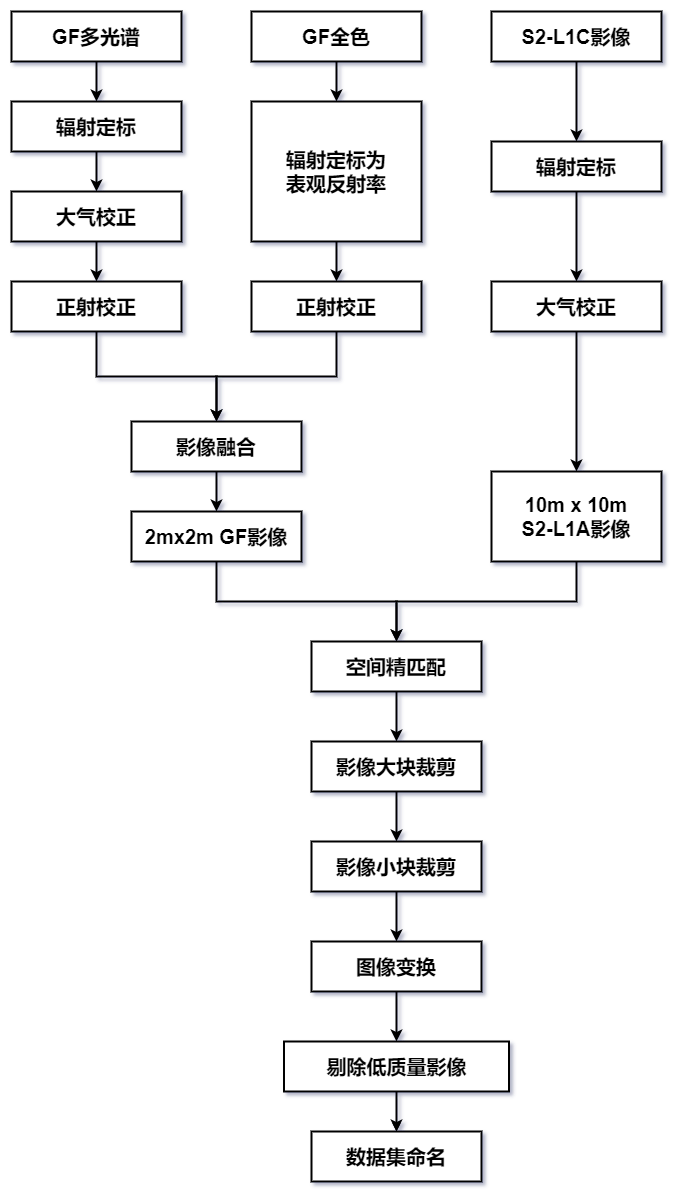
\includegraphics[height=0.7\textheight]{pic/pic0201.png}
    \caption{数据制作流程图}
    \label{fig:0201}
\end{figure}

在之前的制作流程中, 主要分为两大部分. 第一部分主要为ENVI操作, 包括遥感影像预处理, 影像融合, 空间精匹配, 影像大块裁剪; 第二部分为批量处理, 将第一部分得到的大块影像进行小块裁剪, 由于不同源遥感影像存在一定色彩偏差, 需对每对超分影像进行色彩匹配, 对低质量影像(有云雾, 水田变色等情况)进行手动剔除, 将最终得到的高质量影像进行数据集命名, 得到超分影像数据集. 

由于上次制作数据集质量过低, 其表现出问题是, 水田变色, 影像对存在明显差异, 影像块范围较小(100 --> 400), DIV2K数据库都是500-->2000; 其根本原因在于原始遥感影像中, 云雾覆盖较大, 大幅影像裁剪则数据量会少. 超分影像日期为二零二零年四月十六日, 哨兵影像日期为二零二零年四月十九日, 虽然间隔只有短短三天, 但由于天气不同, 水田发生巨大变化, 如~\ref{fig:0202}, 而影像中水田较多. 这导致在剔除低质量影像的工作量过大. 

\begin{figure}[!htbp]
    \centering
    \subfloat[GF]{\label{fig:0202a}
    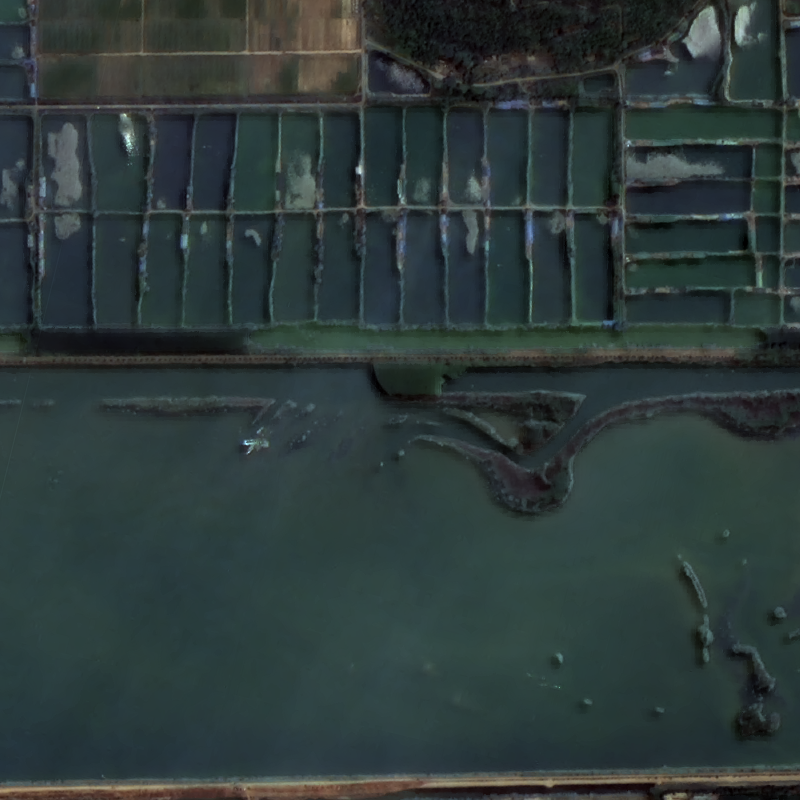
\includegraphics[height=10em]{pic/pic0203.png}}
    \quad
    \subfloat[S2]{\label{fig:0202b}
    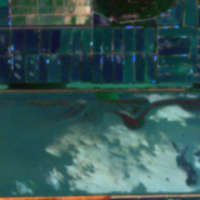
\includegraphics[height=10em]{pic/pic0202.png}}
    \caption{水田对比}
    \label{fig:0202}
\end{figure}

本周在进行新的数据集制作中, 发现原始遥感影像质量高, 数据制作的工作量可大大减少.
\begin{itemize}
    \item 选取云雾遮挡少的高质量影像
    \item 选取城市多, 水田范围小的影像
    \item 可在欧空局直接选择预处理过的L1A级影像
\end{itemize}

由此看来, 上次制作的数据集如~\ref{fig:0203}所示, 可发现, 大量又分散的云, 不适合做超分影像对; 本次如~\ref{fig:0204}所示, 晴空万里, 且欧空局能放在服务器中的L1A影像多数质量较高, 可以信赖:
\begin{figure}[!htbp]
    \centering
    \subfloat[GF]{\label{fig:0203a}
    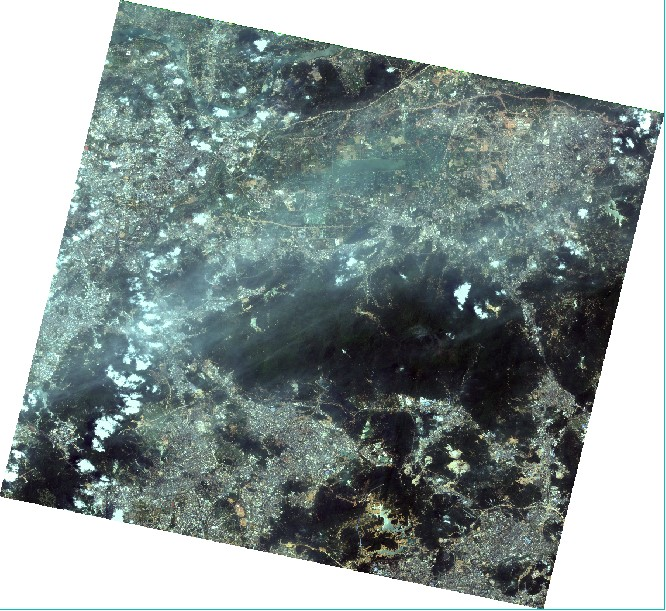
\includegraphics[height=12em]{pic/pic0204gf02.jpg}}
    \qquad
    \subfloat[S2]{\label{fig:0203b}
    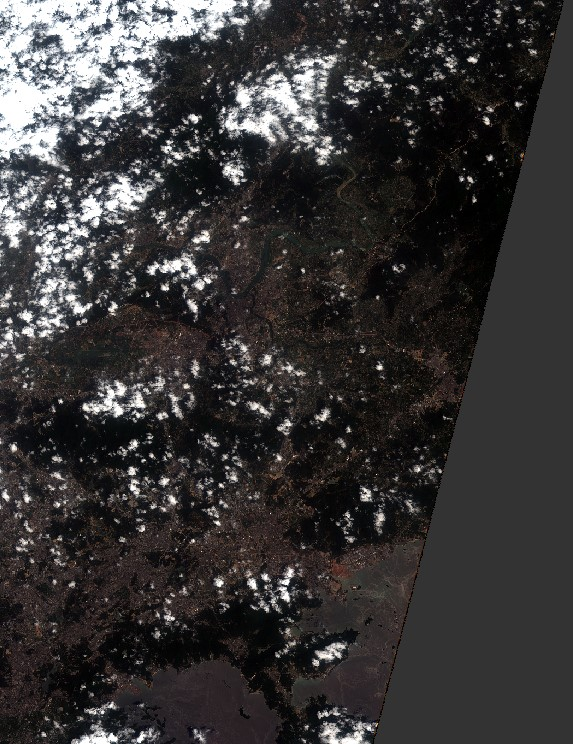
\includegraphics[height=12em]{pic/pic0204s202.jpg}}
    \caption{上次实验原始影像}
    \label{fig:0203}
\end{figure}

\begin{figure}[!htbp]
    \centering
    \subfloat[GF]{\label{fig:0204a}
    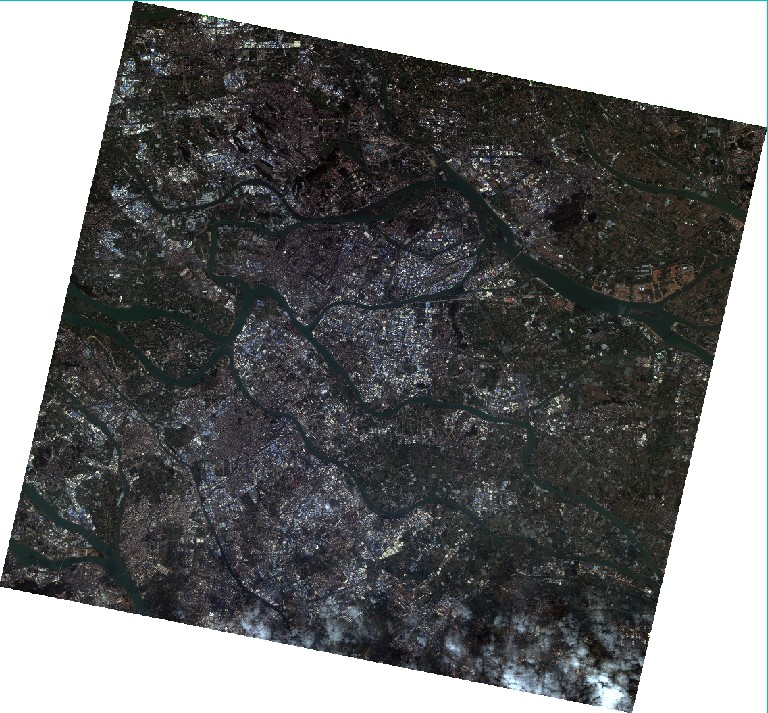
\includegraphics[height=12em]{pic/pic0204gf01.jpg}}
    \qquad
    \subfloat[S2]{\label{fig:0204b}
    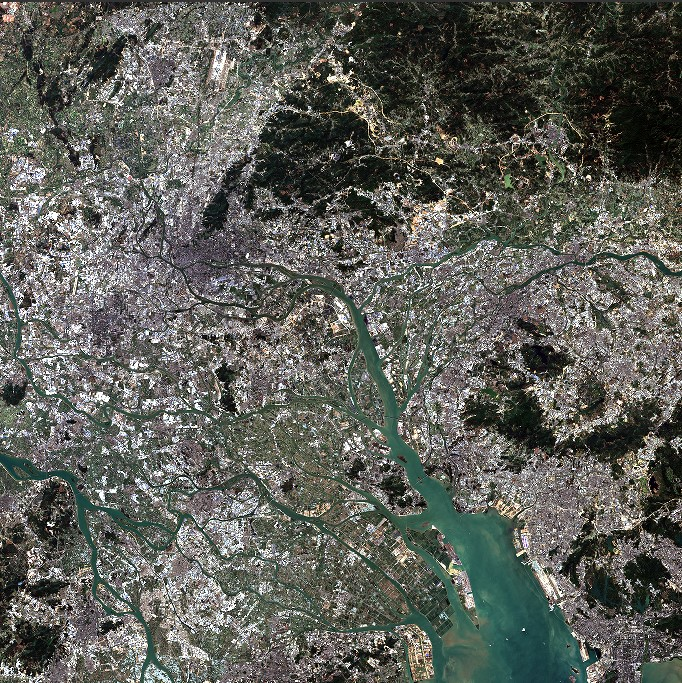
\includegraphics[height=12em]{pic/pic0204s201.jpg}}
    \caption{本次实验原始影像}
    \label{fig:0204}
\end{figure}

充分说明一点:
\begin{quotation}
    \Large
    \itshape
    \centering  
    选择大于努力
\end{quotation}

% \begin{figure}[!htbp]
%     \centering
%     \subfloat[BC]{\label{fig:0105a}
%     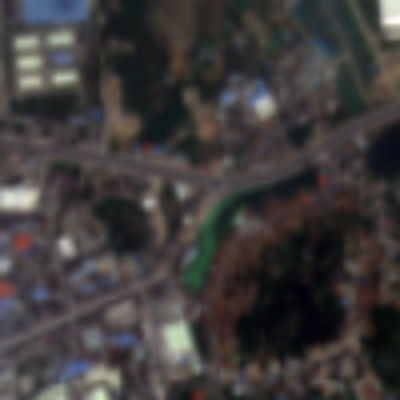
\includegraphics[height=10em]{pic/img5_LR_bicubic.jpg}}
%     \quad
%     \subfloat[SR]{\label{fig:0105b}
%     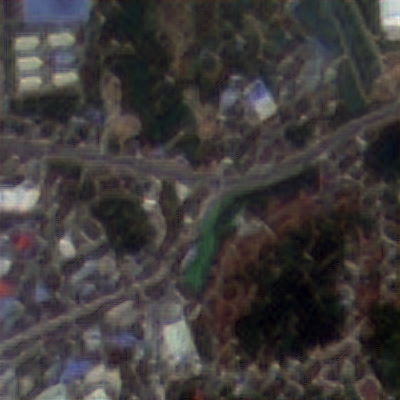
\includegraphics[height=10em]{pic/img5_SR.jpg}}
%     \quad
%     \subfloat[GT]{\label{fig:0105c}
%     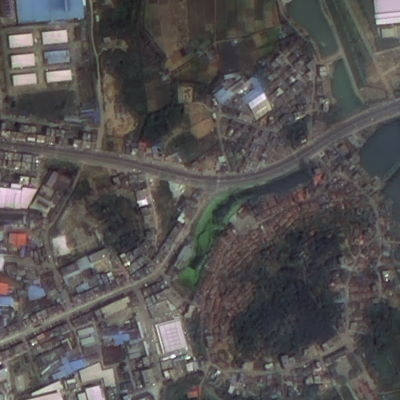
\includegraphics[height=10em]{pic/img5_GT.jpg}}
%     \caption{result05}
%     \label{fig:0105}
% \end{figure}